\documentclass[12pt]{article}
\usepackage{amsmath}
\usepackage{graphicx}
\textwidth15.0cm      
\textheight23.0cm     
\oddsidemargin1.0cm
\evensidemargin0.13cm 
\topmargin-0.325cm    
\parskip1.0ex
\parindent0.0cm
\linespread{1.3}
\usepackage[T2A]{fontenc}
\usepackage[utf8]{inputenc}
%\usepackage[cp1251]{inputenc}
\usepackage[english,russian]{babel}
\usepackage{float}
\restylefloat{table}
\begin{document}

\section{Сложности моделирования динамики облачного АПС}

В областях распространения кучево-слоистой облачности над океаном скачок температуры, влажности и других скаляров на верхней границе АПС может достигать больших значений. При этом, этот слой ``скачка'' имеет малую мощность в вертикальном направлении и не может быть разрешен явно на конечно-разностной сетке, используемой в климатических моделях. Более того, использование конечно-разностной аппроксимации вертикальной адвекции приводит к размыванию слоя ``скачка''. Очевидно, что тонкий баланс между турбулентным вовлечением, вертикальной адвекцией, микрофизическими и радиационными процессами не может быть адекватно воспроизведен в крупномасштабных моделях при использовании традиционных подходов.

В нескольких работах был предложен и реализован подход, позволяющий преодолеть указанные недостатки. В его основе лежит восстановление подсеточной структуры АПС вблизи его верхней границы, предполагающее бесконечно малую толщину слоя ``скачка''. Далее, на основе восстановленной структуры АПС рассчитываются физически обоснованные тенденции скаляров, обусловленные вовлечением и вертикальной адвекцией.

\section{Вертикалные профили скаляров вблизи верхней границы АПС}

Восстановление подсеточной структуры вертикальных профилей потенциальной температуры, влажности и других скаляров осуществляется следующим образом. 

{\bf Шаг 1.} Самый верхний модельный уровень $k$, полностью находящийся внутри АПС, диагносцируется исходя из условия:
\begin{equation}
\theta_{l,k} < \theta_{l,1} + 0.4 < \theta_{l,k+1}\,\, ,
\end{equation}
где $\theta_l = \theta - L/c_p q_l$ - жидкокапельная эквивалентная потенциальная температуры; $q_l$ - удельная водность облаков; $\theta_{l,1}$ - эквивалентная потенциальная температура на нижнем модельном уровне, ближайшем к подстилающей поверхности.

{\bf Шаг 2.} Мы предполагаем, что высота АПС находится в пределах уровня $k+1$, т.е. $z_{k+1/2} < z_i < z_{k+3/2}$ (см. Рисунок \ref{scheme}), но пока не знаем ее конкретного значения. Таким образом, мы предполагаем, что часть уровня $k+1$ в пределах $z_{k+1/2}<z<z_i$ занята воздухом, относящимся к АПС, а верхняя часть в пределах $z_i < z < z_{k+3/2}$ занята воздухом, относящимся к свободной атмосфере. Для того, чтобы определить точно высоту $z_i$, мы предполагаем следующую подсеточную структуру вертикального профиля скаляра (на примере эквивалентной потенциальной температуры $\theta_l$): от $z_k$ до высоты $z_i$ $\theta_l$ меняется по градиенту в АПС $\gamma_{BL} = (\theta_{l,k} - \theta_{l,k-1})/(z_k - z_{k-1})$, а от высоты $z_i$ до $z_{k+2}$ температура меняется по градиенту в свободной атмосфере $\gamma_{FA} = (\theta_{l,k+3} - \theta_{l,k+2})/(z_{k+3} - z_{k+2})$. Кроме того, необходимо потребовать, чтобы среднее значение скаляра по восстановленному профилю в слое $k+1$ было равно значению скаляра на уровне $k+1$ на модельной сетке, т.е.:
\begin{equation}
 \int_{z_{k+1/2}}^{z_{k+3/2}} \theta_l dz = \theta_{l,k+1} (z_{k+3/2}-z_{k+1/2})
\end{equation}

\begin{figure}
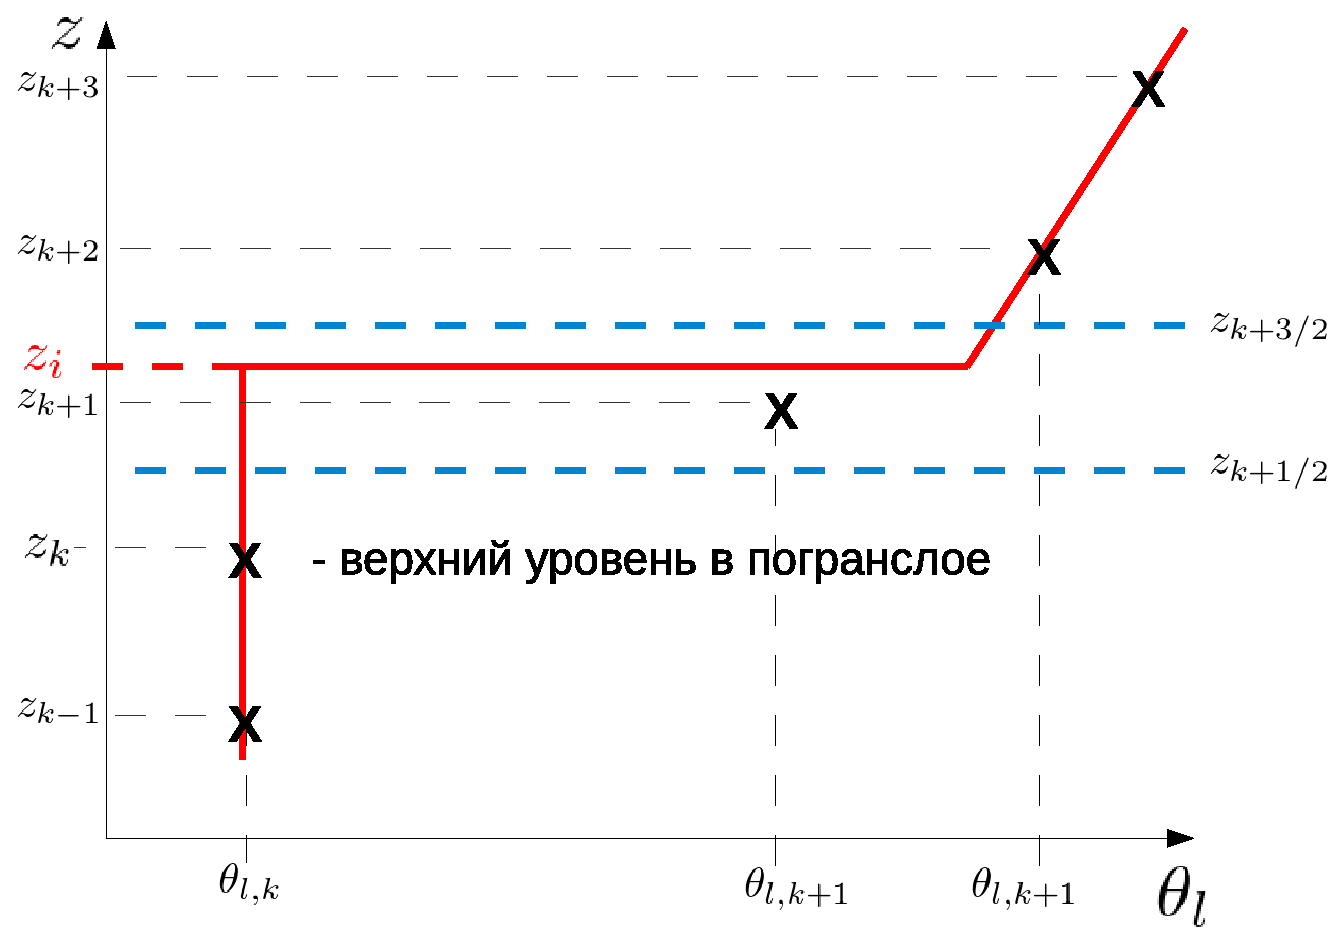
\includegraphics[scale=0.4]{reconstruction.eps}
\caption{Схема построения подсеточной структуры вертикального профиля скаляров на примере жидкокапельной эквивалентной потенциальной температуры $\theta_l$; знаками ``х'' показано положение узлов модельной сетки.}
\label{scheme}
\end{figure}

Учитывая восстановленную структуру вертикального профиля $\theta_l$, интеграл в левой части (2) представим в виде суммы двух интегралов:

\begin{equation} \label{int}
 \int_{z_{k+1/2}}^{z_i} \theta_{l,k} + \gamma_{BL} (z - z_k)  dz + \int_{z_i}^{z_{k+3/2}} \theta_{l,k+2} - \gamma_{FA} (z_{k+2} - z)  dz = \theta_{l,k+1} (z_{k+3/2}-z_{k+1/2})
\end{equation}

После взятия интегралов и приведения подобных получаем квадратное уравнение относительно $\Delta z = z_{k+3/2} - z_i$:

\begin{equation}
a \Delta z^2 + b \Delta z + c = 0
\end{equation}
со следующими коэффициентами
\begin{eqnarray}
a &=& 0.5(\gamma_{fa} - \gamma_{bl}) , \\
b &=& - [\theta_{l,k+2} - \gamma_{fa}(z_{k+2} - z_{k+3/2} )] + [\theta_{l,k} + \gamma_{bl} (z_{k+3/2} - z_k ] , \\
x &=& (z_{k+3/2} - z_{k+1/2})(\theta_{l,k+1} - \theta_k - \gamma_{bl} ( z_{k+1} - z_{k})) 
\end{eqnarray}

\subsection{Тенденции за счет вертикальной адвекции и вовлечения}

С физической точки зрения тенденции скаляров в слое $k+1$, обусловленные вертикальной адвекцией, связаны с изменением во времени высоты АПС в пределах этого слоя. Задача состоит в том, чтобы адекватно воспроизвести этот процесс на конечно-разностной сетке.

Прежде всего, воспользуемся формулой, следующей из уравнения неразрывности и отражающей закон сохранения массы:
\begin{equation} \label{dzdt}
\frac{d z_i}{d t} = w_{z_i} + w_e \,\, ,
\end{equation}
где $w_{z_i}$ - вертикальная скорость; $w_e$ - скорость вовлечения. Если предположить квазиоднородные по горизонтали условия, то полную производную в (\ref{dzdt}) можно заменить на частную.

Далее, продифференцируем по времени уравнение (\ref{int}):
\begin{equation}
\end{equation}

\end{document}
